\documentclass[10pt]{scrbook} \usepackage{modules/nonstahp_book}
\usepackage{mathspec}

\setmainfont[
	Path = f/,
	BoldFont=pb.ttf,
	ItalicFont=pi.ttf,
	BoldItalicFont=pbi.ttf
		]{p.ttf}
\setsansfont[
	Path = f/,
	BoldFont=pb.ttf,
	ItalicFont=pi.ttf,
	BoldItalicFont=pbi.ttf
		]{p.ttf}
		
\setmathfont(Digits)[Path = f/]{p.ttf}
\setmathfont(Latin)[Path = f/]{pi.ttf}
\setmathfont(Greek)[Path = f/, Uppercase]{p.ttf}
\setmathfont(Greek)[Path = f/, Lowercase]{pi.ttf}

\setmonofont[Path = f/]{pmono.ttf}

%\setCJKmainfont[
%	Path=f/,
%	BoldFont=notoserifb.ttf,
%	ItalicFont=notoserifi.ttf,
%	BoldItalicFont=notoserifbi.ttf
%		]{notoserif.ttf}

 \pagestyle{empty}

\captionsetup[figure]{labelformat=empty, labelsep=none}

\begin{document}

\begin{figure} \begin{center}
	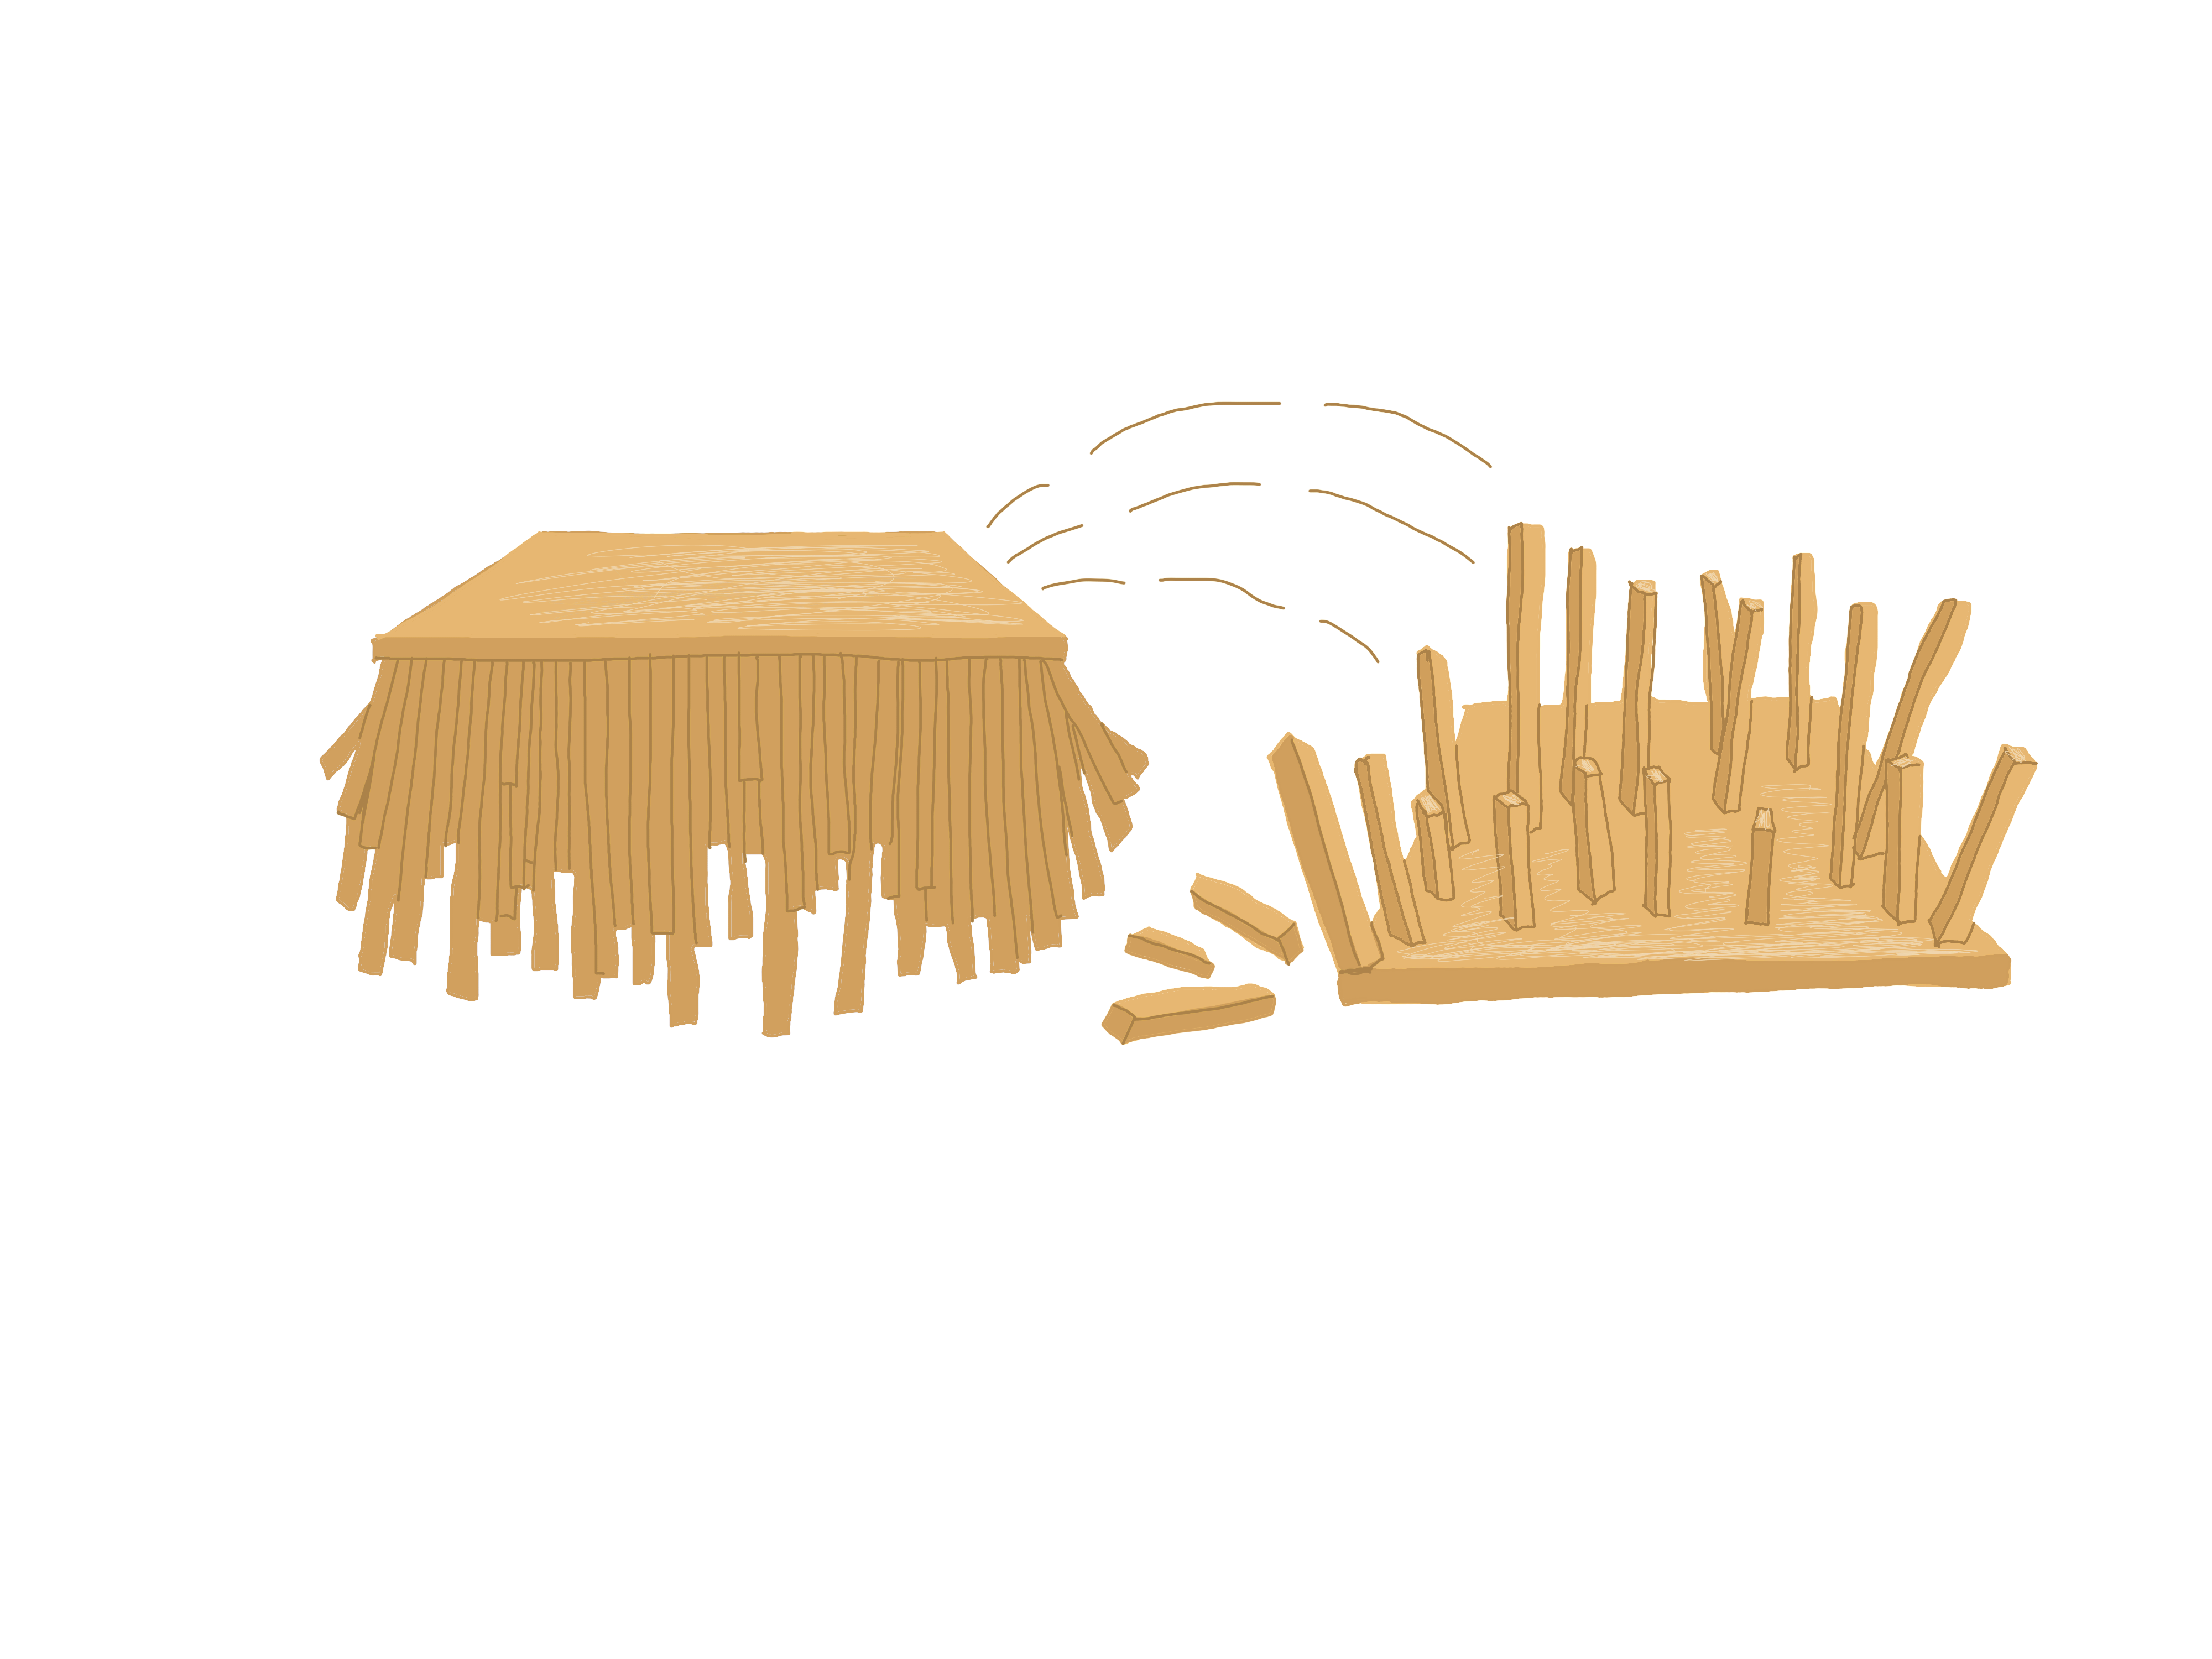
\includegraphics[width=2cm]{figures/color/01}
	%\vspace{1cm}
	\caption{
             {\itshape ... Экспериментальный стул с использованием нанотехнологий 
             (одна из инноваций заключается, например, в том, что у 
             такого стула ровно 720 ножек) падает с лестницы ...}\\
             {Задача 3 <<Современная мебельная фабрика>>, 2018 год, 5 класс.}}
\end{center} \end{figure}

\begin{figure} \begin{center}
	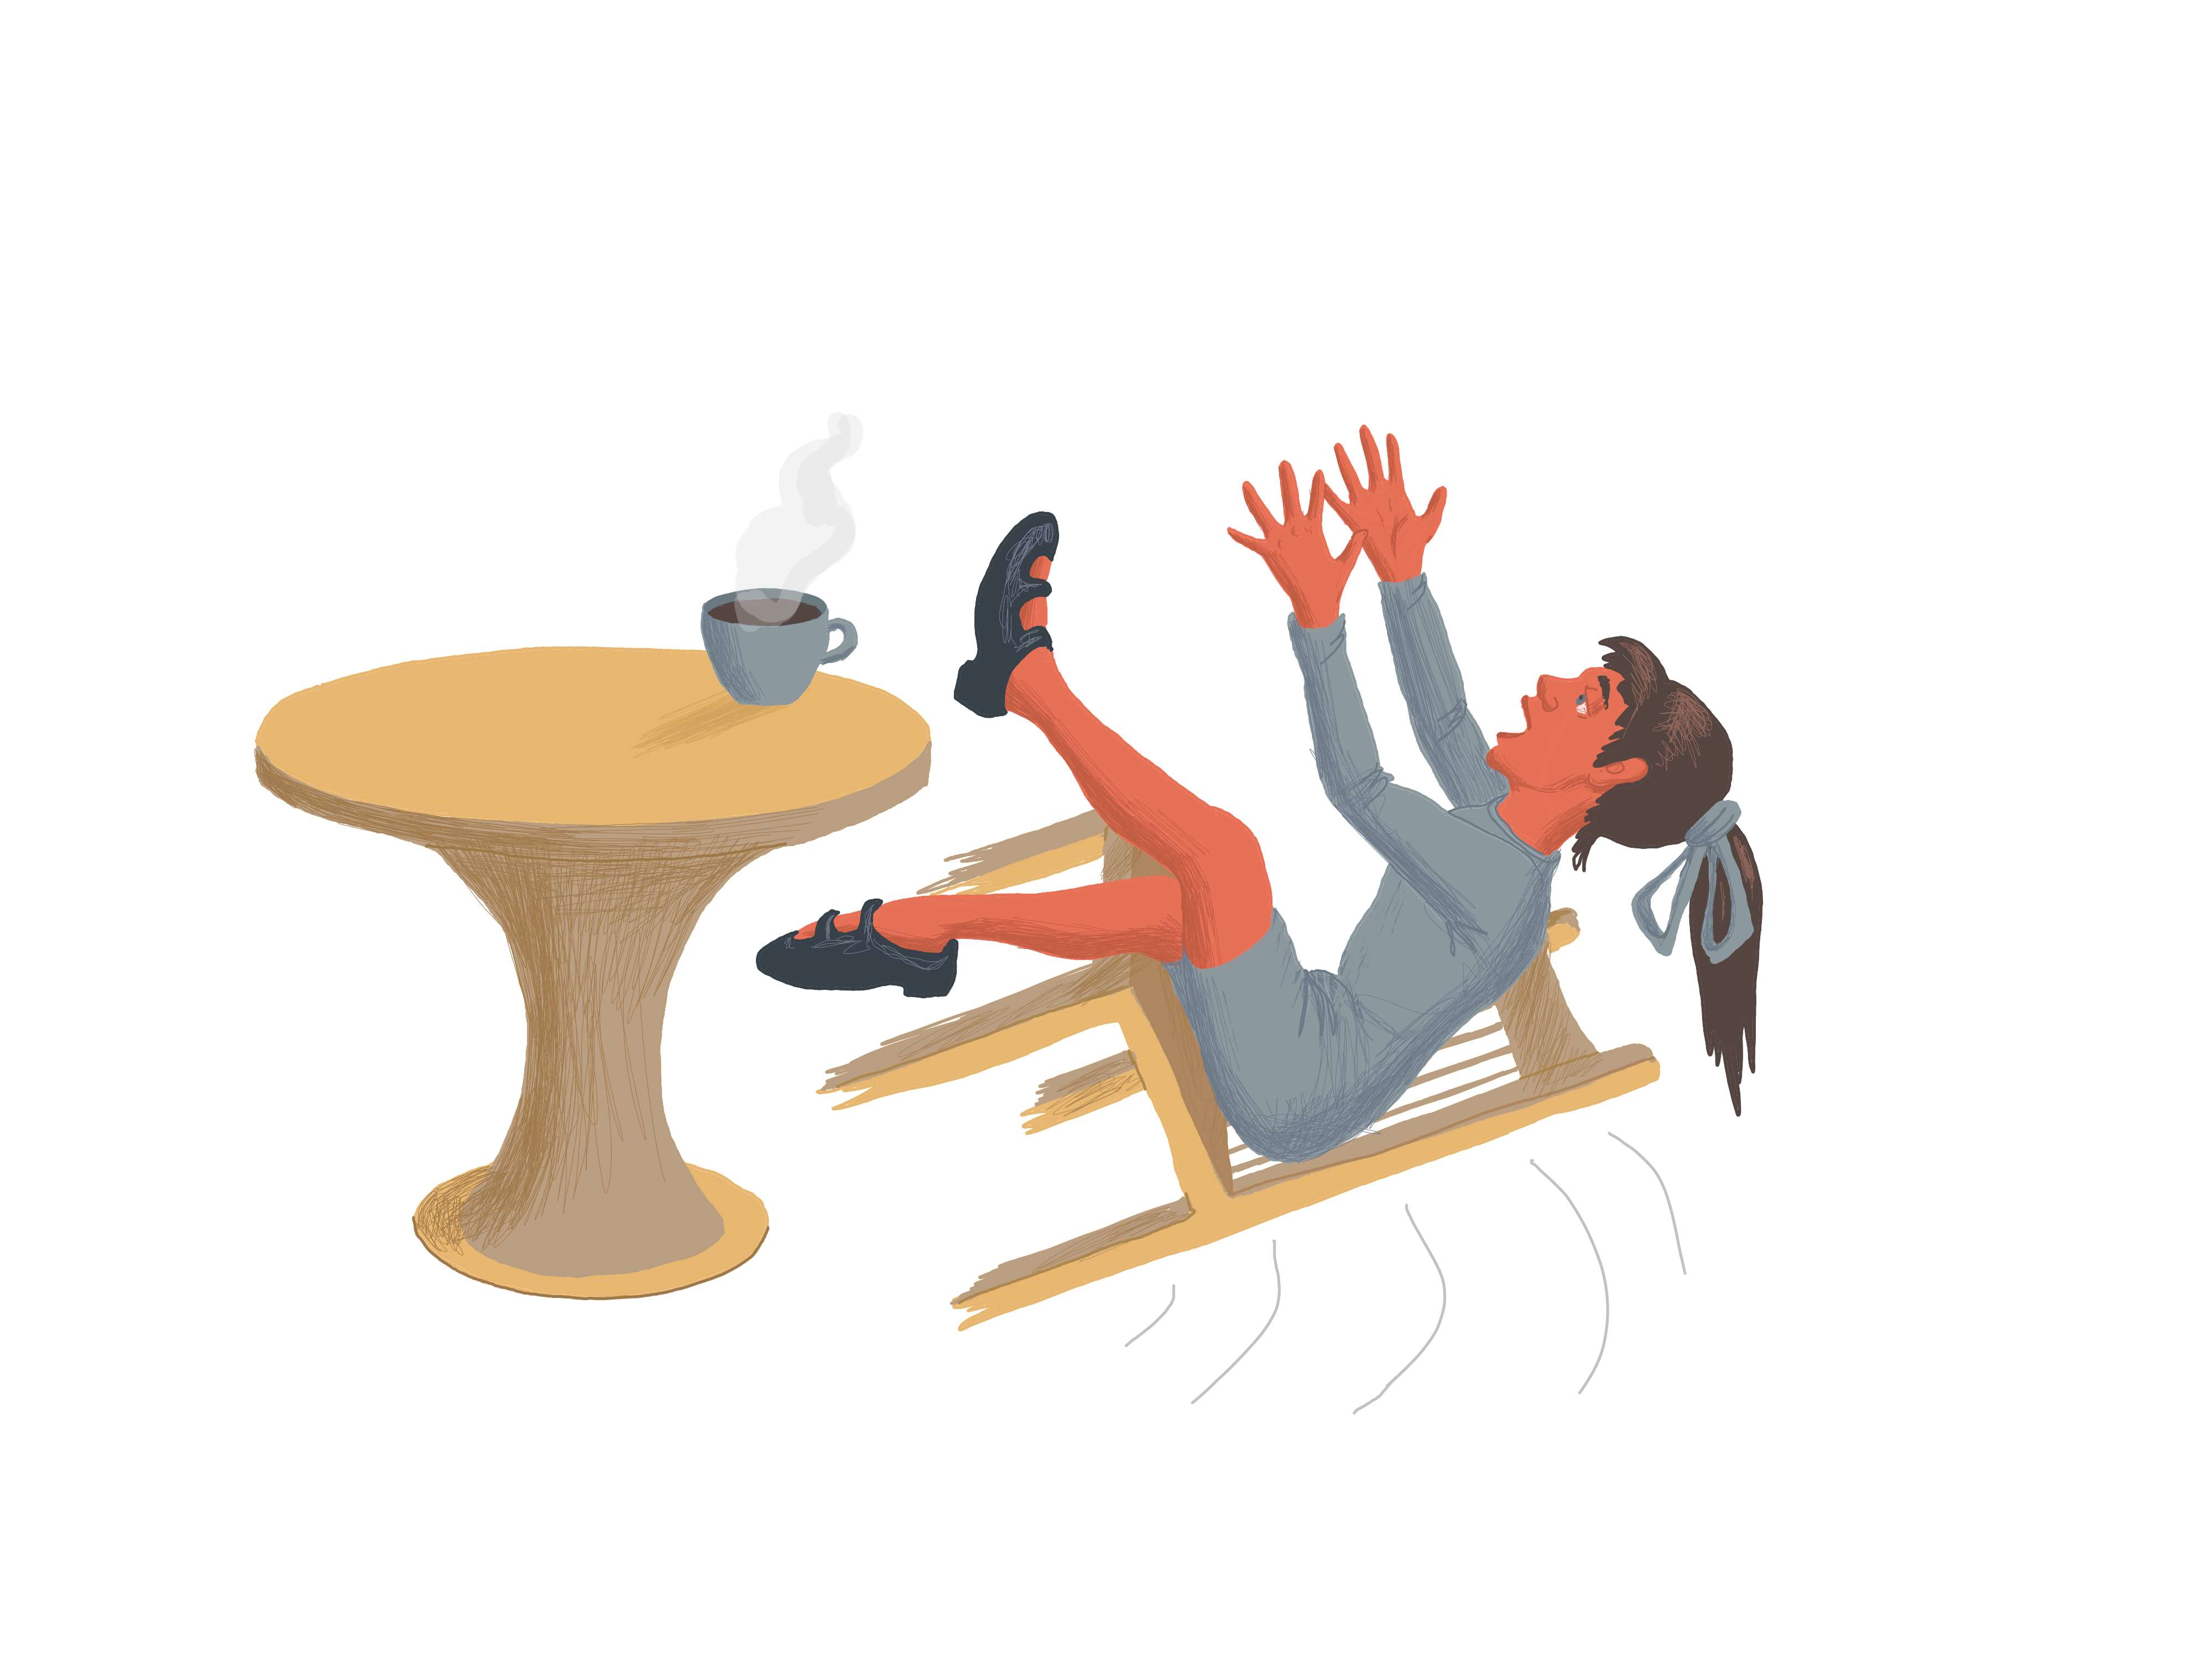
\includegraphics[width=2cm]{figures/color/05}
	%\vspace{1cm}
	\caption{
             {\itshape ... Сколько ножек нужно подпилить Васе, 
              чтобы с утра как минимум $m$ посетителей кафе гарантированно упали? ...}\\
             {Задача 1 <<Падающие стулья>>, 2016 год, 6 класс.}}
\end{center} \end{figure}



\end{document}